\subsection{Data Retrieval and Preprocessing} \label{subsec:data}

For our study we choose two main datasets, each containing gene expression data for healthy and cancerous tissues.
The first one includes healthy tissue data from the Genotype-Tissue Expression (GTEx) project,
and the second one includes cancerous tissue data from the Cell Model Passport (CMP) project.
While these resources are widely used and well-established in research, they do have limitations in terms of their scope and coverage.
The GTEx dataset consists of only adult postmortem donor samples, with 2/3 of them between 50 and 69 years old and 2/3 being male~\cite{GTEX_modelannotation}.
The CMP dataset contains data from donors who are predominantly male (60\%)
and have an age range that is biased towards older adults (50-69 years old)~\cite{CMP_modelannotation}.

The two datasets provide the foundation for our graph database, specifically for the gene nodes.
We aim to create a table with genes as rows,
where each row contains a unique Ensemble ID along with one value representing healthy TPM and another value representing cancerous TPM.
\\


\subsubsection*{GTEx} \label{subsubsec:GTEx}
For the healthy tissue samples used in this study,
we utilize the \texttt{GTEx\_Analysis\_2017-06-05\_v8\_\newline
RNASeQCv1.1.9\_gene\_tpm} dataset from the GTEx portal~\cite{gtex_download}.
The \textbf{GTEx portal} is a large-scale, publicly available resource for studying gene activity.
The Adult GTEx project aims to characterize the gene expression patterns in healthy tissues across different individuals,
providing valuable insights into the underlying biology of human development and disease.

The dataset $A_{orig}$ is in a .gct file format that contains TPM values for 56,156 genes $i$ identified by
Ensemble ID as rows in 17,382 different tissues $j$ as columns (see~\cref{tab:gtex_table}.0).
The data is initially stored in a file in wide format where each tissue $j$ had its own column.
The TPM values for these tissues range between 0 and 747,400.
Since there are no missing values in the dataset, we do not need to handle any missing data.
To process this data into a suitable format, we employ the following steps:

\begin{enumerate}
    \item \textbf{Reshaping to long format:}
    We read the data from the original format in chunks of 3,000 rows at a time due to RAM capacity constraints.
    For each chunk of data, we transform the columns for each tissue $j$ into individual rows,
    resulting in a dataset with three columns and 976,103,592 ($i * j$) rows (see~\cref{tab:gtex_table}.1).

    \item \textbf{Grouping by genes:}
    Once all chunks are processed, we separate the combined dataset again for RAM reasons
    in new chunks of approximately 200 million rows.
    These chunks are grouped by gene using an aggregate function that calculates
    both the sum $S_i$ and count $C_i$ of TPM values for each gene $i$ (see~\cref{tab:gtex_table}.2).

    \item \textbf{Calculating mean TPM:}
    To handle genes that have been split across multiple chunks,
    we performe a global aggregation on the genes of the sum of the dataset.
    Then we calculate the mean TPM value $M_i$ for each gene $i$ by dividing the sum $S_i$ by the count $C_i$
    of each observation (see~\cref{tab:gtex_table}.3).
\end{enumerate}

\begin{table}[h]
    \centering
    \resizebox{\textwidth}{!}{
    \begin{tabular}{|c|c|c|c|}
        \hline
        \textbf{0. Original Format} & \textbf{1. Reshaping to long format} & \textbf{2. Grouping by genes} & \textbf{3. Calculating mean TPM} \\
        \hline
        & & & \\[1mm] % adding more space to the row
        $\begin{aligned}
        i & : \text{gene} \\
        j & : \text{tissue} \\
        a_{ij} & : \text{TPM for gene } i \text{ in tissue } j
        \end{aligned}$ &
        $ A_{\text{long}} = (\text{Gen}_i, \text{Tissue}_j, a_{ij}) $ &
        $ A_{\text{agg}} = (\text{Gen}_i, S_i, C_i )$ &
        $ A_{\text{mean}} = (\text{Gen}_i, M_i )$ \\

        & & & \\[1mm] % adding more space to the row

        & & $ S_i = \sum_{j=1}^{j} a_{ij}, \quad C_i = \sum_{j=1}^{j} 1 $ &
        $ M_i = \frac{S_i}{C_i} $ \\

        & & & \\[1mm] % adding more space to the row

        $ A_{\text{orig}} = \begin{bmatrix}
            a_{11} & a_{12} & \dots & a_{1j} \\
            a_{21} & a_{22} & \dots & a_{2j} \\
            \vdots & \vdots & \ddots & \vdots \\
            a_{i1} & a_{i2} & \dots & a_{ij}
        \end{bmatrix} $ &
        $ A_{\text{long}} = \begin{bmatrix}
            \text{Gen}_1 & \text{Tissue}_1 & a_{11} \\
            \text{Gen}_1 & \text{Tissue}_2 & a_{12} \\
            \vdots & \vdots & \vdots \\
            \text{Gen}_i & \text{Tissue}_j & a_{ij}
        \end{bmatrix} $ &
        $ A_{\text{agg}} = \begin{bmatrix}
            \text{Gen}_1 & S_{1} & C_{1} \\
            \text{Gen}_2 & S_{2} & C_{2} \\
            \vdots & \vdots & \vdots \\
            \text{Gen}_i & S_{i} & C_{i} \\
        \end{bmatrix} $ &
        $ A_{\text{mean}} = \begin{bmatrix}
            \text{Gen}_1 & M_{1}\\
            \text{Gen}_2 & M_{2} \\
            \vdots & \vdots\\
            \text{Gen}_i & M_{i}\\
        \end{bmatrix} $ \\

        & & & \\[1mm] % adding more space to the row
        \hline
        & & & \\[1mm] % adding more space to the row

        % Example Matrix Representation
        $ A_{\text{orig}, i} = \begin{bmatrix}
            8.764 & 0.07187 & \dots & 3.215
        \end{bmatrix}$ &

        $ A_{\text{long}, i} = \begin{bmatrix}
            \text{ENSG...938} & \text{GTEX-111...} & 8.764 \\
            \text{ENSG...938} & \text{GTEX-112...} & 0.07187 \\
            \text{ENSG...938} & \text{GTEX-113...} & 3.215
        \end{bmatrix}$ &

        $ A_{\text{agg}, i} = \begin{bmatrix}
            \text{ENSG...938} & 12.051 & 3
        \end{bmatrix}$ &

        $ A_{\text{mean}, i} = \begin{bmatrix}
            \text{ENSG...938} & 4.017
        \end{bmatrix}$ \\

        & & & \\[1mm] % adding more space to the row
        \hline
    \end{tabular}
    }
    \caption{Data transformation pipeline for the GTEx dataset: Formular and example data per gene}\label{tab:gtex_table}
\end{table}

The resulting dataset (see~\cref{fig:03_01_df_GTEX_healthy_mean}) with 56,156 genes $i$
and a mean TPM value $M_i$ is saved as a CSV file for further processing.\\

\begin{figure}[h]
    \centering
    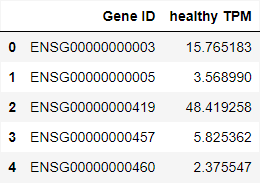
\includegraphics[height=\dfheight]{figures/03_01_GTEX_healthy_mean}
    \caption{Example data of processed GTEx dataset}
    \label{fig:03_01_df_GTEX_healthy_mean}
\end{figure}



%%%%%%%%%%%%%%%%%%%%%%%%%%%%%%%%%%%%%%%%%%%%%%%%%%%%%%%%%%%%%%%%%%%%%%%%%%%%%%%%%%%%%%%%%%%%
% Cell Model Passport
\subsubsection*{CMP} \label{subsubsec:CMP}
For the purpose of the analysis of gene activity in lung cancer, we utilize data from the \textbf{CMP project},
a comprehensive resource for studying cancer-related gene expression.

We obtain the dataset from the CMP portal~\cite{cmp_download} with the name \texttt{rnaseq\_all\_data\_20220624}.
This dataset contains data from the Sanger Institute and the Broad Institute and
consists of a file containing genes associated with diverse cancer types, including lung cancer.
Initially, the data is stored in long format with columns for gene identifiers, tissues, TPM values,
and additional information.

However, the CMP dataset lacks Ensemble IDs, which are crucial for our analysis.
So we need to add the Ensemble IDs to the dataset to ensure consistency and accuracy in our analysis.
To focus on lung cancer-specific data, we load an additional file containing tissue-specific annotations~\cite{cmp_tissue_models}.
Then we filter the CMP dataset to include only tissues from the annotation file with lung cancer as the cancer type.
Specifically, we filter the dataset to include only lung cancer-specific models labeled as
SCLC, NSCLC or Squamous Cell Lung Carcinoma in the $cancer\_type$ column.

The resulting dataset comprises 7,564,389 rows containing genes $i$ and tissues $j$
with associated TPM values for lung cancer (see~\cref{tab:cmp_table}.0).
Specifically, the dataset includes information on 37,262 unique genes $i$ across 203 distinct tissue types $j$.
The dataset contains no missing values and the TPM values span a range of 0 and 132,676.

To prepare the data for further processing, we perform the following steps:
\begin{enumerate}
    \item \textbf{Grouping by genes:}
    We group the dataset by genes to obtain a mean TPM value for every gene.
    This step involves aggregating the data by gene names, resulting in a new dataset
    with a mean TPM value for each gene (see~\cref{tab:cmp_table}.1).

    \item \textbf{Adding Ensembl ID:}
    The original dataset contains own IDs for the genes but lacks the universal Ensembl ID required for matching genes across datasets.
    We overcome this challenge by adding the required Ensembl IDs to our dataset using gene names as a reference point.
    For this purpose we download an Ensemble file from biomart~\cite{bio_marts},
    which contains the Ensembl ID and corresponding name for a gene $x$.

    By analyzing the Ensemble file, we encounter an issue where some gene name were not unique within the file.
    To resolve this problem, we drop all rows with duplicate gene names.
    We then merge the Ensemble table with our CMP data on the gene name to retrieve the Ensemble ID for each gene (see~\cref{tab:cmp_table}.2).

    \item \textbf{Removing missing Ensembl ID:}
    After merging the data, we find that 3,760 of our 37,262 genes still have no Ensembl ID associated with them.
    Since these genes are likely duplicates or do not exist in the Ensemble file,
    we remove them from our dataset to ensure consistency and accuracy of our analysis (see~\cref{tab:cmp_table}.3).
\end{enumerate}

\begin{table}[!h]
    \centering
    \resizebox{\textwidth}{!}{
    \begin{tabular}{|c|c|c|c|}
        \hline
        \textbf{0. Original Format} & \textbf{1. Grouping by genes} & \textbf{2. Adding Ensembl ID} & \textbf{3. Removing missing Ensembl ID} \\
        \hline
        & & & \\[1mm] % adding more space to the row

        % 1. Additional formulars
        $\begin{aligned}
        i & : \text{gene} \\
        j & : \text{tissue} \\
        b_{ij} & : \text{TPM for gene } i \text{ in tissue } j
        \end{aligned}$ &

        $ M_i = \frac{1}{j}\sum_{j=1}^{j} b_{ij} $ &

        $\text{EID}_i =
        \begin{cases}
            \text{EID}_x & \text{if } \exists x \in E_{\text{ens}}: \text{Name}_x = \text{Name}_i, \\
            \text{NULL} & \text{if } \nexists x \in E_{\text{ens}} : \text{Name}_x = \text{Name}_i.
        \end{cases}$ &

        $ B_{\text{clean}} = B_{\text{ens}} \setminus \{ i \mid EID_i = \text{NULL} \} $
        \\

        & & & \\[1mm] % adding more space to the row

        % 2. Row definitions
        $ B_{\text{orig}} = ( \text{ID}_i, \text{Name}_i, \text{Tissue}_j, b_{ij}, \dots) $ &
        $ B_{\text{agg}} =  ( \text{ID}_i, \text{Name}_i, M_i) $ &
        \makecell{$ E_{\text{ens}} =  ( \text{EID}_x, \text{Name}_x) $ \\
            $ B_{\text{ens}} =  ( \text{ID}_i, \text{Name}_i, \text{EID}_i, M_i) $} &
        $ B_{\text{clean}} =  ( \text{ID}_i, \text{Name}_i, \text{EID}_i, M_i) $
        \\

        & & & \\[1mm] % adding more space to the row


        % 3. Style of the Matrix
        $ B_{\text{orig}} = \begin{bmatrix}
            \text{ID}_1 & \text{Name}_1 & \text{Tissue}_1 & b_{11} \\
            \text{ID}_1 & \text{Name}_1 & \text{Tissue}_2 & b_{12} \\
            \vdots & \vdots & \vdots & \vdots \\
            \text{ID}_i & \text{Name}_i & \text{Tissue}_j & b_{ij}
        \end{bmatrix} $ &
        $ B_{\text{agg}} = \begin{bmatrix}
            \text{ID}_1 & \text{Name}_1 & M_{1} \\
            \text{ID}_2 & \text{Name}_2 & M_{2} \\
            \vdots & \vdots & \vdots \\
            \text{ID}_i & \text{Name}_i & M_{i}
        \end{bmatrix} $ &
        $ B_{\text{ens}} = \begin{bmatrix}
            \text{ID}_1 & \text{Name}_1 & \text{EID}_1 & M_{1} \\
            \text{ID}_2 & \text{Name}_2 & NULL &  M_{2} \\
            \vdots & \vdots & \vdots & \vdots \\
            \text{ID}_i & \text{Name}_i & \text{EID}_i & M_{i}
        \end{bmatrix} $ &
        $ B_{\text{clean}} = \begin{bmatrix}
            \text{ID}_1 & \text{Name}_1 & \text{EID}_1 & M_{1} \\
            \text{ID}_3 & \text{Name}_3 & \text{EID}_3 & M_{3} \\
            \vdots & \vdots & \vdots & \vdots \\
            \text{ID}_i & \text{Name}_i & \text{EID}_i & M_{i}
        \end{bmatrix} $
        \\


        & & & \\[1mm] % adding more space to the row
        \hline
        & & & \\[1mm] % adding more space to the row

        % 4. Example Matrix for a single gene
        $ B_{\text{org}, i} = \begin{bmatrix}
            \text{SIDG...16} & \text{CASP10} & \text{SIDM...13} & 14.41 \\
            \text{SIDG...16} & \text{CASP10} & \text{SIDM...61} & 0.64 \\
            \text{SIDG...16} & \text{CASP10} & \text{SIDM...50} & 3.26
        \end{bmatrix}$ &
        $ B_{\text{agg}, i} = \begin{bmatrix}
            \text{SIDG...16} & \text{CASP10} & 5.017
        \end{bmatrix}$ &
        $ B_{\text{ens}, i} = \begin{bmatrix}
            \text{SIDG...16} & \text{CASP10} & \text{ENSG...400} & 5.017
        \end{bmatrix}$ &
        $ B_{\text{clean}, i} = \begin{bmatrix}
            \text{SIDG...16} & \text{CASP10} & \text{ENSG...400} & 5.017
        \end{bmatrix}$
        \\


        & & & \\[1mm] % adding more space to the row
        \hline
    \end{tabular}
    }
    \caption{Data transformation pipeline for the CMP dataset: Formular and example data per gene}\label{tab:cmp_table}
\end{table}


The resulting dataset (\cref{fig:03_01_df_CMP_cancer_mean}) contains 33,502 genes with mean TPM values for lung cancer and
is saved as a CSV file for further processing.

\begin{figure}[h]
    \centering
    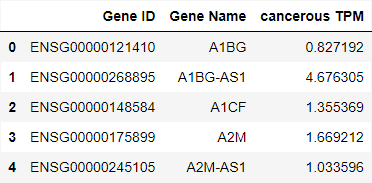
\includegraphics[height=\dfheight]{figures/03_01_CMP_cancer_mean}
    \caption{Example data of processed CMP dataset}
    \label{fig:03_01_df_CMP_cancer_mean}
\end{figure}